%\documentclass[conference]{IEEETran}
\documentclass{article}
% Packages to draw tables
\usepackage{booktabs} % for \toprule, \midrule and \bottomrule (improved \hline)
\usepackage{multirow}
% Packages to generate figures
\usepackage{graphicx}

\begin{document}
\title{This is a Personal \LaTeXe{} Template}
\maketitle

\section{Introduction}
\label{sec:intr}
This is an introduction. It references the work~\cite{shannon2001mathematical}.

\section{Method}
\label{sec:method}
This is the method.

\section{Experiment}
\label{sec:exp}
This is the experiment.

\subsection{Table}
\begin{table}[h] % table position: here
  \centering     % center of the page
  \caption[table1]{A table of numbers and colors}
  \label{tab:color_num_table}

  \begin{tabular}{rlcr} % four columns aligned as right, left, center and right
    \toprule
    \multirow{2}{*}{No.} & First  & Second & Third  \\
                         & Column & Column & Column \\
    \midrule

    1 & one & two & three \\

    \midrule
    \multicolumn{3}{l}{Colors} \\
    \midrule

    2 & red & blue & green                     \\
    3 & red & \multicolumn{2}{c}{multi-colors} \\
    \bottomrule
  \end{tabular}
\end{table}

\subsection{Figure}
\begin{figure}
  \centering
  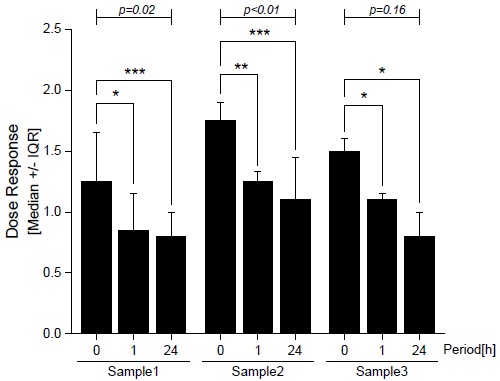
\includegraphics[scale=0.4]{fig/fig1.png}
  \caption{Dose responses from different samples}
  \label{fig:dose_response}
\end{figure}

\section{Discussion}
\label{sec:result}
This is the discussion from Section~\ref{sec:exp}

% \bibliographystyle{IEEETran}
\bibliographystyle{abbrv}
\bibliography{ref}


\end{document}
